\documentclass[aspectratio=169,11pt]{beamer}
\usepackage[T1]{fontenc}
\usepackage[utf8]{inputenc}
\usepackage{lmodern}
\usepackage{booktabs}
\usepackage{graphicx}
\usepackage{amsmath}
\definecolor{navy}{HTML}{14263F}
\definecolor{teal}{HTML}{087F8C}
\definecolor{soft}{HTML}{F1F5F8}
\setbeamercolor{structure}{fg=teal}
\setbeamercolor{frametitle}{fg=white,bg=navy}
\setbeamercolor{title}{fg=white}
\setbeamercolor{normal text}{fg=navy}
\setbeamercolor{block title}{fg=white,bg=teal}
\setbeamercolor{block body}{fg=navy,bg=soft}
\setbeamertemplate{navigation symbols}{}
\setbeamertemplate{footline}{\hfill\color{teal}\insertframenumber\,/\,\inserttotalframenumber\hspace{1em}\vspace{0.6em}}
\setbeamertemplate{itemize items}[circle]
\title{A Comparative Study of Data Generation Strategies\\for Imbalanced Classification}
\subtitle{Synthetic, Simulated, and Augmented Data}
\author{Author information to be added}
\date{Conference presentation draft \textbullet\ October 2026}
\begin{document}
	{\setbeamercolor{background canvas}{bg=navy}\begin{frame}[plain]\titlepage\end{frame}}
	\begin{frame}{Research question}\Large\centering Does changing the minority-class training distribution improve out-of-sample ranking?\vspace{1em}\begin{block}{Hypothesis under examination}\normalsize Data-generation and reweighting strategies may help, but benefits are not guaranteed across data geometry, shift, and classifier choice.\end{block}\end{frame}
	\begin{frame}{Compared strategies}\begin{itemize}\setlength\itemsep{0.65em}\item \textbf{Baseline:} original training data, no intervention\item \textbf{Class weighting:} modify loss contribution, not observations\item \textbf{SMOTE:} interpolate minority-class neighbors\item \textbf{CTGAN:} learned conditional tabular generator\item \textbf{Oracle simulation:} minority observations from known synthetic mechanism\end{itemize}\vspace{0.5em}\footnotesize Oracle sampling is an experimental reference, not a deployable real-data oracle.\end{frame}
	\begin{frame}{Five evaluation scenarios}\begin{tabular}{@{}ll@{}}\toprule Scenario & Characterization\\\midrule S1 & Overlapping class distributions\\ S2a & Nonlinear concentric rings, lower noise\\ S2b & Nonlinear concentric rings, higher noise\\ S3a & Test shift in a nuisance variable\\ S3b & Test shift in an informative variable\\\bottomrule\end{tabular}\vspace{1em}\begin{block}{Learners}Logistic regression (LR) and random forest (RF).\end{block}\end{frame}
	\begin{frame}{Experimental protocol}\begin{columns}[T]\begin{column}{0.5\textwidth}\begin{block}{Per evaluation seed}\begin{itemize}\item Fit: 750 observations\item Validation: 250 observations\item Test: 2,000 observations\item 30 independent evaluation seeds\end{itemize}\end{block}\end{column}\begin{column}{0.48\textwidth}\begin{block}{Leakage control}\begin{itemize}\item Augment fitting split only\item Keep validation and test untouched\item CTGAN epochs chosen on separate development seeds\item Freeze epoch count at 10\end{itemize}\end{block}\end{column}\end{columns}\vspace{0.8em}\centering\large $5\ \text{scenarios}\times 30\ \text{seeds}\times 5\ \text{methods}\times 2\ \text{models}\times 2\ \text{threshold policies}=3{,}000$\end{frame}
	\begin{frame}{Primary endpoint and inference}\begin{itemize}\setlength\itemsep{0.7em}\item \textbf{Average Precision (AP)}: primary, threshold-independent metric\item Paired within seed, scenario and learner: $\Delta AP=AP_{\mathrm{method}}-AP_{\mathrm{baseline}}$\item 40 contrasts: 5 scenarios $\times$ 2 learners $\times$ 4 alternatives\item Two-sided paired $t$ tests; \textbf{Holm} correction across all 40 tests\item 95\% confidence intervals shown in the analysis are \textbf{unadjusted}\end{itemize}\end{frame}
	\begin{frame}{Main finding}\begin{columns}[c]\begin{column}{0.45\textwidth}\centering\Huge\color{teal}25/40\\[0.4em]\normalsize Holm-significant AP differences\\[1em]\Huge\color{navy}0\\[0.4em]\normalsize significant improvements over baseline\end{column}\begin{column}{0.53\textwidth}\begin{block}{Direction of evidence}\large All 25 significant differences favored the \textbf{baseline}.\end{block}\vspace{0.7em}\small No conclusion of universal inferiority is warranted outside the evaluated conditions.\end{column}\end{columns}\end{frame}
	\begin{frame}{Average AP differences by strategy}\centering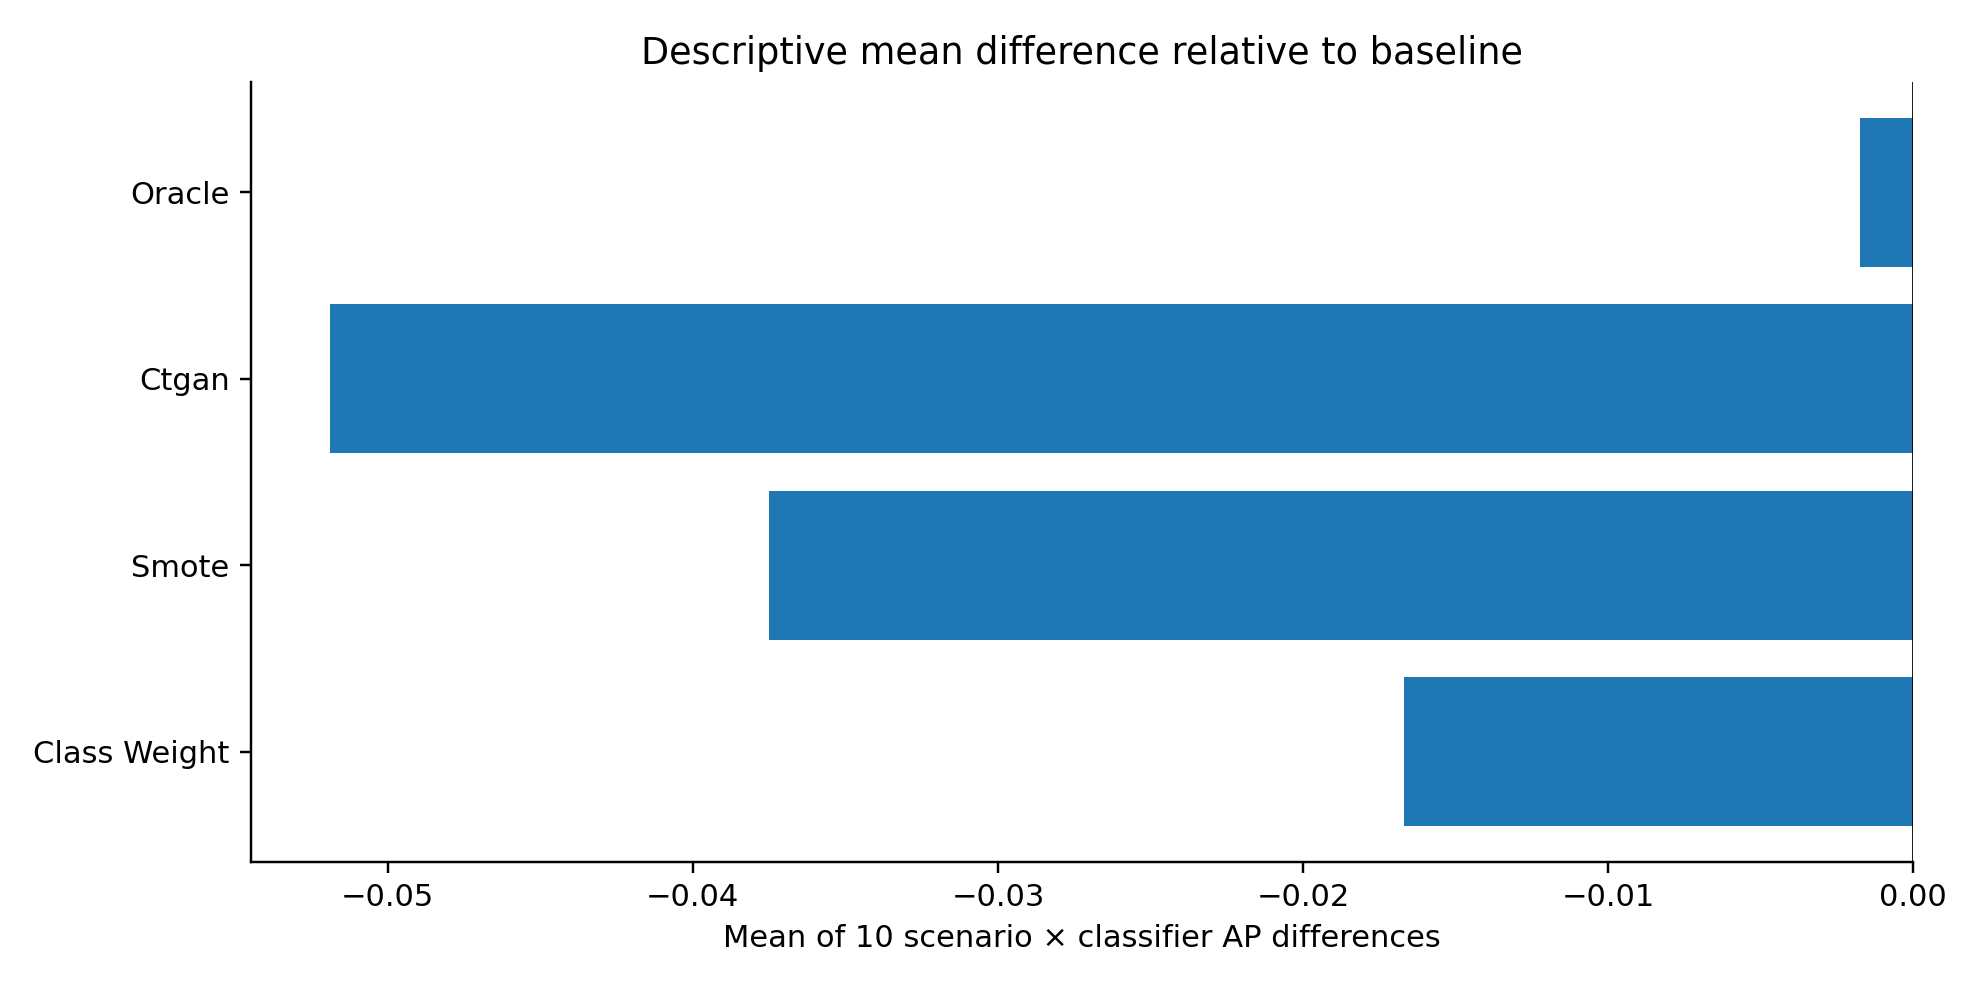
\includegraphics[width=0.91\linewidth,height=0.77\textheight,keepaspectratio]{figure_3_method_summary.png}\\\scriptsize Descriptive means across ten scenario--classifier combinations; not pooled significance tests.\end{frame}
	\begin{frame}{Where performance changes}\centering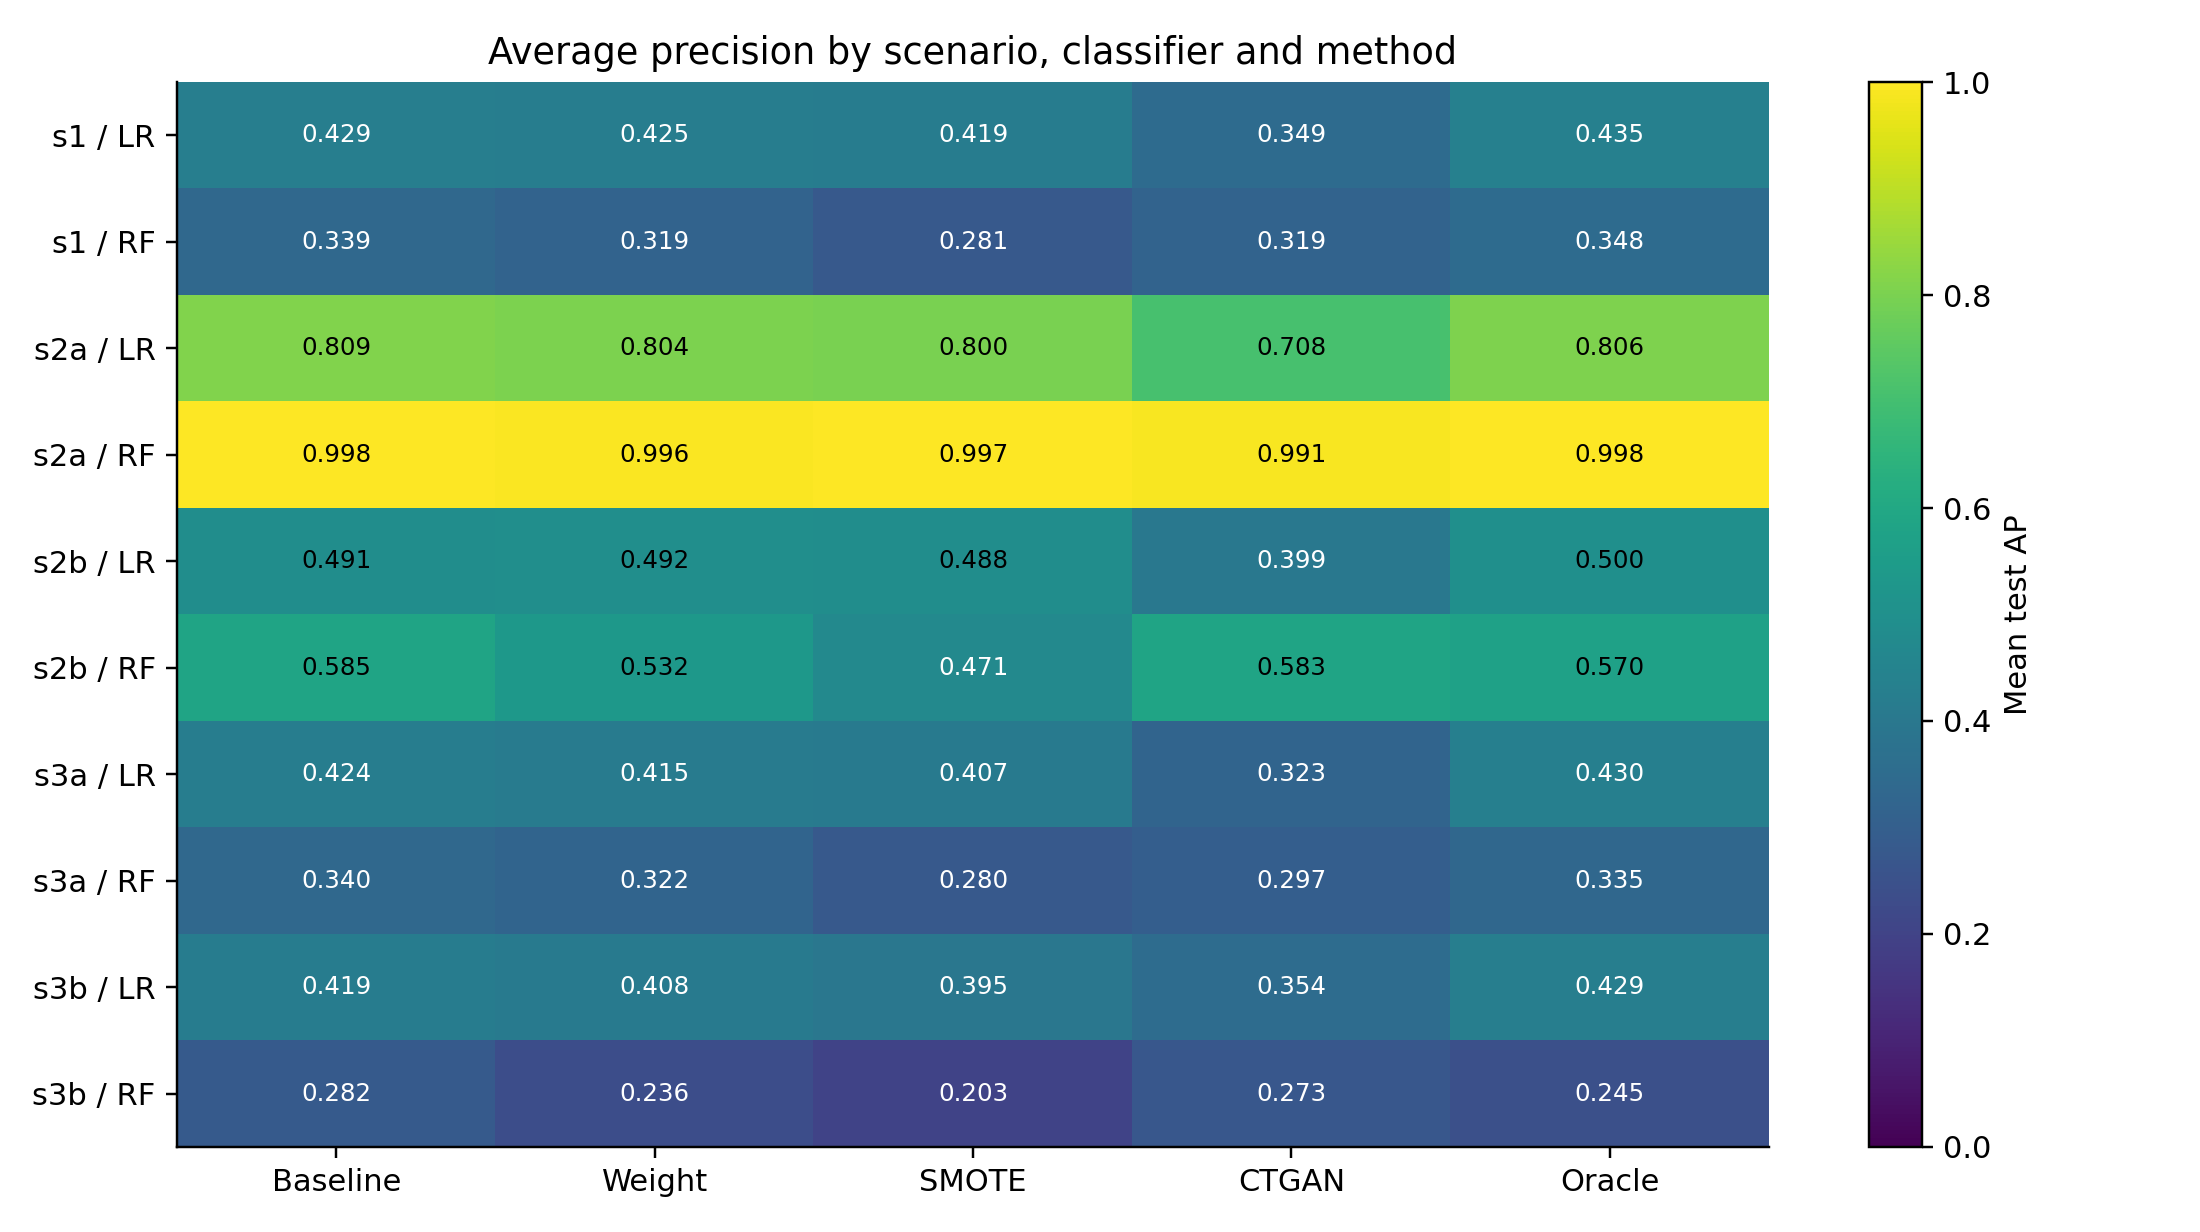
\includegraphics[width=0.93\linewidth,height=0.78\textheight,keepaspectratio]{figure_2_ap_heatmap.png}\end{frame}
	\begin{frame}{Paired effects across conditions}\centering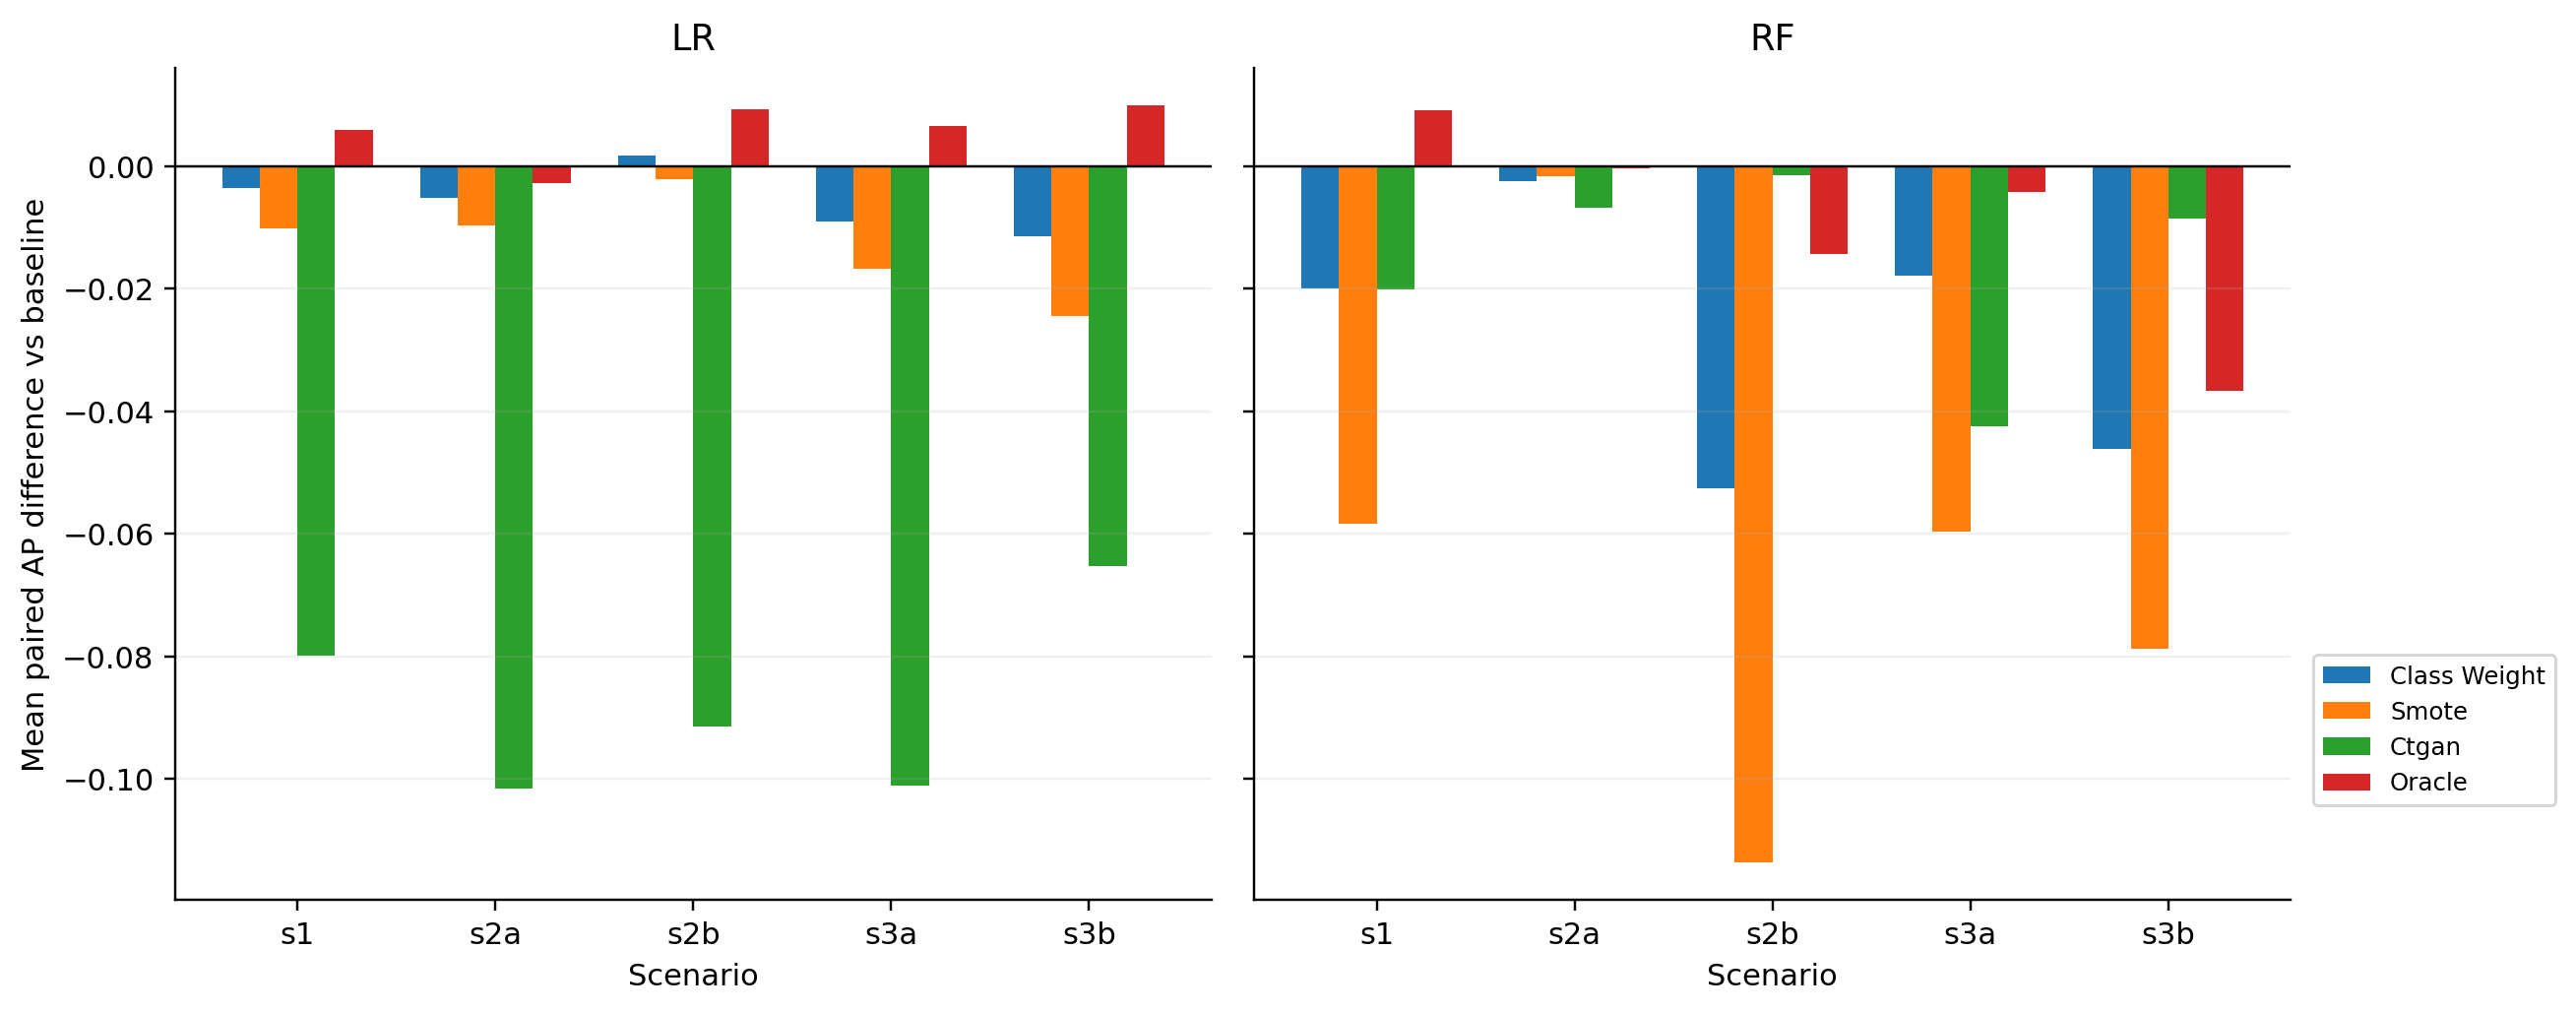
\includegraphics[width=0.95\linewidth,height=0.78\textheight,keepaspectratio]{figure_1_ap_differences.png}\end{frame}
	\begin{frame}{Method-level summary}\centering\begin{tabular}{@{}lrr@{}}\toprule Strategy & Mean $\Delta AP$ & Significant losses / 10\\\midrule Class weighting & $-0.0167$ & 6\\ SMOTE & $-0.0375$ & 9\\ CTGAN & $-0.0519$ & 8\\ Oracle simulation & $-0.0018$ & 2\\\bottomrule\end{tabular}\vspace{1em}\begin{block}{Interpretation}\small Oracle simulation remained closest to baseline on average, while SMOTE and CTGAN frequently reduced AP. Responses were heterogeneous by scenario and classifier.\end{block}\end{frame}
	\begin{frame}{Why might augmentation hurt?}\begin{itemize}\setlength\itemsep{0.8em}\item Interpolation may create samples that do not respect complex class boundaries.\item A learned generator can reproduce training patterns without improving test ranking.\item Reweighting changes the optimization target, not necessarily ranking quality.\item Distribution shift can make additional minority observations less representative.\end{itemize}\vspace{0.7em}\footnotesize These are plausible explanations, \emph{not} causally established mechanisms in this experiment.\end{frame}
	\begin{frame}{Limitations and reproducibility}\begin{itemize}\setlength\itemsep{0.65em}\item Synthetic scenarios; no external real-world validation\item Fixed sample sizes, classifier choices and generation settings\item AP is primary; threshold-dependent outcomes are secondary\item Structural fidelity and runtime were \textbf{not} measured in the delivered result archive\item 30-seed paired analysis with 40-test multiplicity correction\end{itemize}\end{frame}
	\begin{frame}{Conclusions}\begin{block}{Take-home message}\large More minority-class samples do not automatically mean better ranking performance.\end{block}\vspace{1em}\begin{itemize}\item Evaluate augmentation against a strong untouched-data baseline.\item Separate model selection from confirmatory evaluation.\item Report negative findings and adjust for multiple comparisons.\item Validate on real-world datasets before generalizing.\end{itemize}\end{frame}
	\begin{frame}{Recent research: 2023--2026}
		\small
		\begin{itemize}\setlength\itemsep{0.65em}
			\item \textbf{Kotelnikov et al. (2023, ICML):} TabDDPM extends tabular generation beyond GANs to diffusion models.
			\item \textbf{D'souza et al. (2025, AAAI):} Explicitly modeling class-overlap regions can improve synthetic-data utility for imbalanced classification.
			\item \textbf{Won et al. (2026, Electronics):} Compared SMOTE, CTGAN, TVAE and Gaussian Copula on imbalanced real-world tabular data; reported gains in recall and F1.
			\item \textbf{G\"und\"uz and \c{S}ahin (2026, Applied Sciences):} Compared SMOTE, CTGAN, TVAE and TabDDPM in a biological application.
		\end{itemize}
		\vspace{0.3em}\scriptsize These papers provide context, not direct replications: datasets, endpoints and protocols differ.
	\end{frame}
	\begin{frame}{Positioning our findings against recent work}
		\small\begin{block}{Why results need not agree}
			Reported gains in \textbf{recall/F1} do not imply gains in \textbf{average precision (AP)}; the metric, data geometry, learner and validation protocol all matter.
		\end{block}
		\begin{itemize}\setlength\itemsep{0.65em}
			\item Our study isolates five controlled scenarios with 30 paired seeds and Holm correction across 40 AP contrasts.
			\item Recent studies broaden the range of generators and real-world domains; they do not establish universal benefits.
			\item Future external validation should include real datasets, stronger generator tuning, runtime and fidelity measurements.
		\end{itemize}
	\end{frame}
	\begin{frame}{References: foundations and methods}
		\tiny\begin{itemize}\setlength\itemsep{0.5em}
			\item Chawla, N. V., et al. (2002). SMOTE: Synthetic Minority Over-sampling Technique. \emph{JAIR}, 16, 321--357.
			\item He, H., and Garcia, E. A. (2009). Learning from Imbalanced Data. \emph{IEEE TKDE}, 21(9), 1263--1284.
			\item Xu, L., et al. (2019). Modeling Tabular Data using Conditional GAN. \emph{NeurIPS}.
			\item Saito, T., and Rehmsmeier, M. (2015). The Precision-Recall Plot Is More Informative than the ROC Plot. \emph{PLOS ONE}, 10(3), e0118432.
			\item Holm, S. (1979). A Simple Sequentially Rejective Multiple Test Procedure. \emph{Scandinavian Journal of Statistics}, 6(2), 65--70.
			\item Kotelnikov, A., et al. (2023). TabDDPM: Modelling Tabular Data with Diffusion Models. \emph{ICML}, PMLR 202, 17564--17579.
		\end{itemize}
		\tiny\begin{itemize}\setlength\itemsep{0.8em}
			\item D'souza, A., M, S., and Sarawagi, S. (2025). Synthetic Tabular Data Generation for Imbalanced Classification: The Surprising Effectiveness of an Overlap Class. \emph{AAAI}, 39(15), 16127--16134. DOI: 10.1609/aaai.v39i15.33771.
			\item Won, D.-H., Shin, K.-S., and Youm, S. (2026). Synthetic Data Augmentation for Imbalanced Tabular Data: A Comparative Study of Generation Methods. \emph{Electronics}, 15(4), 883. DOI: 10.3390/electronics15040883.
			\item G\"und\"uz, A. F., and \c{S}ahin, C. B. (2026). Synthetic Data Augmentation for Imbalanced Tabular Protein Subcellular Localization: A Comparative Study of SMOTE, CTGAN, TVAE, and TabDDPM Methods. \emph{Applied Sciences}, 16(8), 3694. DOI: 10.3390/app16083694.
			\item Kurakova, A., and Homayouni, H. (2025). A comprehensive evaluation framework for synthetic medical tabular data generation. \emph{Journal of Biomedical Informatics}, 171, 104939. DOI: 10.1016/j.jbi.2025.104939.
		\end{itemize}
	\end{frame}
	\begin{frame}[plain]\centering\vspace{2cm}{\Huge\color{teal}Thank you}\\[1em]{\Large Questions and discussion}\end{frame}
\end{document}